%++++++++++++++++++++++++++++++++++++++++
% Don't modify this section unless you know what you're doing!
\documentclass[letterpaper,12pt]{article}
\usepackage{tabularx} % extra features for tabular environment
\usepackage{amsmath}  % improve math presentation
\usepackage{graphicx} % takes care of graphic including machinery
\usepackage[margin=1in,letterpaper]{geometry} % decreases margins
\usepackage{cite} % takes care of citations
\usepackage[final]{hyperref} % adds hyper links inside the generated pdf file
\usepackage{pgfplotstable, booktabs}
\usepackage{placeins}
\usepackage{tabularray}
\usepackage{titlesec}
\usepackage{fancyhdr}
\usepackage{empheq}
\usepackage{amssymb}
\usepackage{sectsty}
\usepackage{tcolorbox}
\usepackage{listings}
\usepackage{xcolor}
\usepackage{parskip}
\usepackage{cancel}
\usepackage{enumitem}
\usepackage{amsmath}
\usepackage{mathrsfs}
\usepackage{physics}
\usepackage{subcaption}
\usepackage{pdfpages}
\usepackage{amsthm} 
\usepackage{color}
\usepackage{import}

%\graphicspath{{Questions/Figures}}

\definecolor{codegreen}{rgb}{0,0.6,0}
\definecolor{codegray}{rgb}{0.5,0.5,0.5}
\definecolor{codepurple}{rgb}{0.58,0,0.82}

\lstdefinestyle{mystyle}{
    commentstyle=\color{codegreen},
    keywordstyle=\color{codepurple},
    numberstyle=\tiny\color{codegray},
    stringstyle=\color{codegreen},
    basicstyle=\ttfamily\small,
    breakatwhitespace=false,         
    breaklines=true,                 
    captionpos=b,                    
    keepspaces=true,                                                     
    showspaces=false,                
    showstringspaces=false,
    showtabs=false,                  
    tabsize=4
}

\lstset{style=mystyle}
  
\newcommand*\widefbox[1]{\fbox{\hspace{0em}#1\hspace{0em}}}
%define a divergence command which does \text{div}
\DeclareMathOperator{\Div}{Div}


\pagestyle{fancy}
\fancyhf{} % Clear all header and footer fields
\fancyhead[L]{MEC E 430}
%\fancyhead[C]{Center Header} 
\fancyhead[C]{Assignment 1}
\fancyhead[R]{Alex Diep}

\fancyfoot[C]{\thepage}

\pgfplotsset{compat=1.18} 
\titleformat*{\section}{\Large\bfseries}
\titleformat*{\subsection}{\large\bfseries}

\renewcommand{\thesection}{Question \arabic{section}}
\renewcommand{\thesubsection}{(\alph{subsection})}
\renewcommand*{\arraystretch}{1.5}

\hypersetup{
	colorlinks=true,       % false: boxed links; true: colored links
	linkcolor=blue,        % color of internal links
	citecolor=blue,        % color of links to bibliography
	filecolor=magenta,     % color of file links
	urlcolor=blue         
}
%++++++++++++++++++++++++++++++++++++++++
\begin{document}
% \begin{titlepage}
%     \centering
%     \vspace*{2cm} % Adjust vertical spacing
    
%     % Title
%     \Huge {MEC E 301 \\Lab 1: Dimensional Measurement} \\
%     \vspace{1cm} % Adjust vertical spacing
    
%     % Author
%     \Large by: Alex Diep \\
%     \vspace{1cm} % Adjust vertical spacing

%     % Date
%     \Large Date: September 19, 2023 \\ % or manually specify a date
%     \vspace{4cm} % Adjust vertical spacing

%     % CCID and Student ID in smtaller font
%     \normalsize CCID: abdiep \\
%     \normalsize Student ID: 1664334 \\ 
%     \normalsize Section: D21 \\
    
%     \vfill % Fill vertical space
    
%     % Additional content (e.g., university logo or other information)
    
% \end{titlepage}

\section{}

% Consider the Blasius solution for a laminar flat plate boundary layer. The 
% nondimensional slope at the wall is given by equation 1 below. 
% (
% 𝑑(𝑢/𝑈)
% 𝑑𝜂 )
% 𝜂=0
% = 𝑓
% ′′(0) = 0.332 (Eq. 1)
% Transform this result to physical variables and show that the following equation
% is correct. 
% 𝜏𝑤 = 0.332 ∙
% 𝜌𝑈
% 2
% √𝑅𝑒𝑥
% (Eq. 2)

\textit{Consider the Blasius solution for a laminar flat plate boundary layer. The nondimensional slope at the wall is given by equation 1 below.}
\begin{equation}
    \left. \frac{d(u/U)}{d\eta} \right|_{\eta=0} = f''(0) = 0.332 \label{eq:1}
\end{equation}

\textit{Transform this result to physical variables and show that the following equation is correct.}
\begin{equation}
    \tau_w = 0.332 \cdot \rho U^2 \sqrt{Re_x} \label{eq:2}
\end{equation}

\textbf{Solution}

At the wall, we specify that the shear stress is given by
\begin{align}
    \tau_w &= \mu \left( \frac{du}{dy} \right)_{y=0}  \label{eq:wallshear}
\end{align}
From the Blasius, 
\begin{align*}
    \eta &= y \sqrt{\frac{U}{\nu x}} \\
    \implies d \eta &= \sqrt{\frac{U}{\nu x}} dy \\
    \eta = 0 &\implies y = 0
\end{align*}
Then,
\begin{align*}
    \frac{d f'}{d\eta} &= \frac{d (u/U)}{d\eta} \\
    &= \frac{d (u/U)}{dy \sqrt{\frac{U}{\nu x}}} \\
    &= \frac{du}{dy} \frac{1}{U} \sqrt{\frac{\nu x}{U}} 
\end{align*}
Then from the solution,
\begin{align*}
    \left. \frac{d(u/U)}{d\eta} \right|_{\eta=0} &= 0.332 \\
    &= \left. \frac{du}{dy} \right|_{y=0} \frac{1}{U} \sqrt{\frac{\nu x}{U}}
\end{align*}
Solving for $\left. \frac{du}{dy} \right|_{y=0}$,
\begin{align*}
    \implies \left. \frac{du}{dy} \right|_{y=0} &= 0.332 U \sqrt{\frac{U}{\nu x}} 
\end{align*}
Substituting this into (\ref{eq:wallshear}),
\begin{align*}
    \tau_w &= \mu \left. \frac{du}{dy} \right|_{y=0} \\
    &= \mu \cdot 0.332 U \sqrt{\frac{U}{\nu x}} \\
    &= 0.332 U \sqrt{\frac{\mu^2 U}{\frac{\mu}{\rho}x}} \\
    &= 0.332 U \sqrt{\frac{\mu \rho U}{x} \cdot \frac{\rho U}{\rho U}} \\
    &= 0.332 U \sqrt{\rho^2 U^2 \cdot \frac{\mu}{\rho U x}} \\
    &= \boxed{0.332 \frac{\rho U^2}{\sqrt{\text{Re}_x}}}
\end{align*}
Thus, we have shown that equation (\ref{eq:2}) is correct.
\section{}
% In order to avoid boundary layer interference, engineers design a “boundary layer 
% scoop” to skim off the boundary layer in a large wind tunnel (see Figure 1). The 
% scoop is constructed of thin sheet metal. The air is at 20°C and flows at 𝑉 =
% 45.0 m/s. How high (dimension ℎ) should the scoop be at downstream distance 
% 𝑥 = 1.45 m?

\textit{In order to avoid boundary layer interference, engineers design a “boundary layer scoop” to skim off the boundary layer in a large wind tunnel (see Figure 1). The scoop is constructed of thin sheet metal. The air is at 20°C and flows at $V = 45.0 m/s$. How high (dimension $h$) should the scoop be at downstream distance $x = 1.45 m$?}

\begin{figure}[H]
    \centering
    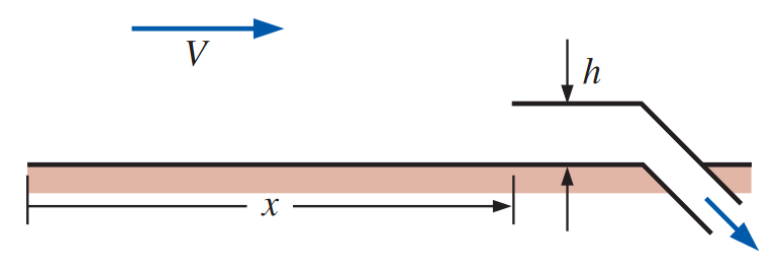
\includegraphics[width=0.5\textwidth]{Questions/Figures/Q2 Problem Diagram.png}
    \caption{Boundary Layer Scoop}
\end{figure}

First, calculate the Reynolds number at $x = 1.45 m$. The kinematic viscosity of air at $20^\circ C$ is $\nu = 1.516 \times 10^{-5} m^2/s$ \cite{cengel_fluid_2018}.
\begin{equation*}
    \text{Re}_x = \frac{Vx}{\nu} = \frac{45.0 \times 1.45}{1.516 \times 10^{-5}} = 4.30 \times 10^6
\end{equation*}
This is past the $\text{Re}_{\text{engineer}} = 5 \times 10^5$ threshold, so this is turbulent. Using the turbulent boundary layer thickness equation,
\begin{align*}
    \frac{\delta}{x} &= \frac{0.16}{\text{Re}_x^{1/7}} \\
    &= \frac{0.16}{(4.30 \times 10^6)^{1/7}} \\
    &= 0.0181 \times 10^{-3} 
\end{align*}
Then,
\begin{align*}
    \delta &= 0.0181 \times 10^{-3} \times 1.45 \\
    &= 2.62 \times 10^{-5} \\
    &= \boxed{26.2 \text{ mm}}
\end{align*}
So the scoop should be at least 26.2 mm high at $x = 1.45$m.
\section{}
% The streamwise velocity component of a steady, incompressible, laminar, flat 
% plate boundary layer of boundary layer thickness 𝛿 is approximated by the simple 
% linear expression, 𝑢 = 𝑈𝑦/𝛿 for 𝑦 < 𝛿, and 𝑢 = 𝑈 for 𝑦 > 𝛿 (see Figure 2). 
% Generate expressions for displacement thickness and momentum thickness as 
% functions of 𝛿, based on this linear approximation. Compare the approximate 
% values of 𝛿
% ∗
% /𝛿 and 𝜃/𝛿 to the values of 𝛿
% ∗
% /𝛿 and 𝜃/𝛿 obtained from the Blasius 
% solution.

\textit{The streamwise velocity component of a steady, incompressible, laminar, flat plate boundary layer of boundary layer thickness $\delta$ is approximated by the simple linear expression, $u = Uy/\delta$ for $y < \delta$, and $u = U$ for $y > \delta$ (see Figure \ref{fig:q3_flat_plate}). Generate expressions for displacement thickness and momentum thickness as functions of $\delta$, based on this linear approximation. Compare the approximate values of $\delta^*/\delta$ and $\theta/\delta$ to the values of $\delta^*/\delta$ and $\theta/\delta$ obtained from the Blasius solution.}
\begin{figure}[H]
    \centering
    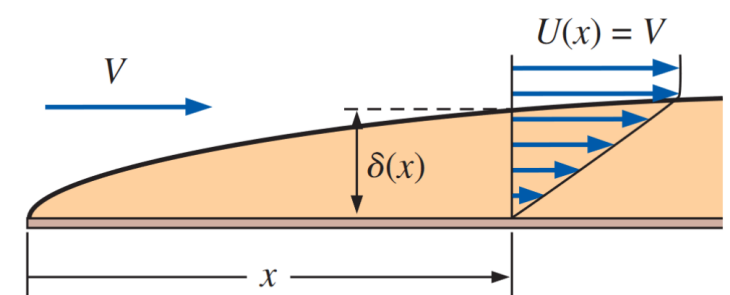
\includegraphics[width=0.5\textwidth]{Questions/Figures/Q3 Problem Diagram.png}
    \caption{Flat Plate Boundary Layer}
    \label{fig:q3_flat_plate}
\end{figure}

By conservation of mass, 
\begin{align*}
    \delta^* &= \int_{0}^{\delta} \left( 1 - \frac{y}{\delta} \right) dy \\
    &= \left[ y - \frac{y^2}{2\delta} \right]_{0}^{\delta} \\
    &= \delta - \frac{\delta^2}{2\delta} \\
    &= \frac{\delta}{2}
\end{align*}
or more conveniently,
\begin{align*}
    \Aboxed{\frac{\delta^*}{\delta} &= \frac{1}{2}}
\end{align*}
By conservation of momentum,
\begin{align*}
    \theta &= \int_{0}^{\delta} \frac{u}{U} \left( 1 - \frac{u}{U} \right) dy \\
    &= \int_{0}^{\delta} \frac{y}{\delta} \left( 1 - \frac{y}{\delta} \right) dy \\
    &= \int_{0}^{\delta} \left( \frac{y}{\delta} - \frac{y^2}{\delta^2} \right) dy \\
    &= \left[ \frac{y^2}{2\delta} - \frac{y^3}{3\delta^2} \right]_{0}^{\delta} \\
    &= \frac{\delta^2}{2\delta} - \frac{\delta^3}{3\delta^2} \\
    &= \frac{\delta}{2} - \frac{\delta}{3} \\
    &= \frac{\delta}{6}
\end{align*}
or more conveniently,
\begin{align*}
    \Aboxed{\frac{\theta}{\delta} &= \frac{1}{6}}
\end{align*}
Recall from the Blasius solution for laminar boundary layers on a flat plate,
\begin{align*}
    \frac{\delta}{x} &= \frac{4.91}{\sqrt{\text{Re}_x}} \\
    \frac{\delta^*}{x} &= \frac{1.72}{\sqrt{\text{Re}_x}} \\
    \frac{\theta}{x} &= \frac{0.664}{\sqrt{\text{Re}_x}}
\end{align*}
Then,
\begin{empheq}[box=\fbox]{align*}
    \frac{\delta^*}{\delta} &= \frac{1.72}{4.91} = 0.350 \\
    \frac{\theta}{\delta} &= \frac{0.664}{4.91} = 0.135
\end{empheq}
The relative errors are then,
\begin{empheq}[box=\fbox]{align*}
    \text{Error}_{\delta^*} &= \frac{0.350 - 0.5}{0.350} \times 100\% = 42.9\% \\
    \text{Error}_{\theta} &= \frac{0.135 - 0.166}{0.135} \times 100\% = 23.0\%
\end{empheq}
The approximation is not very accurate, with high errors in both $\delta^*$ and $\theta$.
\section{}
% The 𝑢 velocity component of a steady, two-dimensional, incompressible flow 
% field is 𝑢 = 3𝑎𝑥
% 2 − 2𝑏𝑥𝑦, where 𝑎 and 𝑏 are constants. Velocity component 𝑣
% is unknown. Generate an expression for 𝑣 as a function of 𝑥 and 𝑦
The $u$ velocity component of a steady, two-dimensional, incompressible flow field is $u = 3ax^2 - 2bxy$, where $a$ and $b$ are constants. The velocity component $v$ is unknown. Generate an expression for $v$ as a function of $x$ and $y$.

\subsection*{Solution}
The continuity equation for incompressible flow is given by
\begin{align*}
    \nabla \cdot \vec{v} &= 0 \\
    \frac{\partial u}{\partial x} + \frac{\partial v}{\partial y} &= 0
\end{align*}
Substituting the given expression for $u$ into the continuity equation, we have
\begin{align*}
    \frac{\partial}{\partial x}(3ax^2 - 2bxy) + \frac{\partial v}{\partial y} &= 0 \\
    6ax - 2by + \frac{\partial v}{\partial y} &= 0 
\end{align*}
Solving for $v$, we have
\begin{align*}
    \frac{\partial v}{\partial y} &= 2by - 6ax \\
    \Aboxed{v &= by^2 - 6axy + g(x)}
\end{align*}

\section{}
% An aircraft is designed to cruise at Mach number Ma = 1.1 at 12,000 m where 
% the atmospheric temperature is 236.15 K. Determine the stagnation temperature 
% on the leading edge of the wing

\textit{An aircraft is designed to cruise at Mach number Ma = 1.1 at 12,000 m where the atmospheric temperature is 236.15 K. Determine the stagnation temperature on the leading edge of the wing.}

\textbf{Solution}

Assume
\begin{itemize}
    \item The flow is steady, adiabatic, and one dimensional
    \item Isentropic flow
    \item Air is an ideal gas with properties $c_p = 1.005 kJ/(kg \cdot K)$, $k = 1.4$, and $R = 287 J/(kg \cdot K)$
\end{itemize}
First we need to find the speed of air. For an ideal gas,
\begin{align*}
    c &= \sqrt{kRT} \\
    \text{Ma} &= \frac{V}{c} \\
    \implies V &= \text{Ma} \cdot c \\
    &= \text{Ma} \sqrt{kRT} 
\end{align*}
Then,
\begin{align*}
    V &= 1.1 \sqrt{1.4 \cdot 287 \cdot 236.15} \\
    &= 338.8376 \text{ m/s}
\end{align*}
Stagnation temperature is then,
\begin{align*}
    T_0 &= T + \frac{V^2}{2c_p} \\
    &= 236.15 + \frac{(338.8376)^2}{2(1.005) \cdot 1000} \\
    &= \boxed{293.27 \text{ K}}
\end{align*}
\section{}
% An ideal gas with 𝑘 = 1.4 is flowing through a nozzle such that the Mach 
% number is 1.6 where the flow area is 45 cm2
% . Approximating the flow as 
% isentropic, determine the flow area at the location where the Mach number is 
% 0.8

\textit{An ideal gas with $k = 1.4$ is flowing through a nozzle such that the Mach number is 1.6 where the flow area is $45 cm^2$. Approximating the flow as isentropic, determine the flow area at the location where the Mach number is 0.8.}

\textbf{Solution}
Assume
\begin{itemize}
    \item The flow is steady, adiabatic, and one dimensional
    \item Isentropic flow
    \item Air is an ideal gas
\end{itemize}

The relation between flow area to throat area is given by 
\begin{align*}
    \frac{A_1}{A^\star} &= \frac{1}{\text{Ma}} \left[ \frac{2}{k+1} \left( 1 + \frac{k-1}{2} \text{Ma}^2 \right) \right]^{(k+1)/(2(k-1))} \\
    &= \frac{1}{1.6} \left[ \frac{2}{1.4+1} \left( 1 + \frac{1.4-1}{2} (1.6)^2 \right) \right]^{(1.4+1)/(2(1.4-1))} \\
    &= 1.250235
\end{align*}
Then,
\begin{align*}
    A^\star &= \frac{45}{1.250235} \\
    &= 35.993 \text{ cm}^2
\end{align*}
Then using the same relation, but with $\text{Ma} = 0.8$,
\begin{align*}
    \frac{A_2}{A^\star} &= \frac{1}{0.8} \left[ \frac{2}{1.4+1} \left( 1 + \frac{1.4-1}{2} (0.8)^2 \right) \right]^{(1.4+1)/(2(1.4-1))} \\
    &= 1.03823
\end{align*}
Then,
\begin{align*}
    A_2 &= 35.993 \times 1.03823 \\
    &= \boxed{37.376 \text{ cm}^2}
\end{align*}
\section{}
% steady, two-dimensional, incompressible flow field in the 𝑥𝑦-plane has a 
% stream function given by ψ = 𝑎𝑥
% 2 − 𝑏𝑦
% 2 + 𝑐𝑥 + 𝑑𝑥𝑦, where 𝑎, 𝑏, 𝑐, and 𝑑 are 
% constants. 
% (a) Obtain expressions for velocity components 𝑢 and 𝑣,
% (b)Verify that the flow field satisfies the incompressible continuity equation.
A steady, two-dimensional, incompressible flow field in the $xy$-plane has a stream function given by $\psi = ax^2 - by^2 + cx + dxy$, where $a$, $b$, $c$, and $d$ are constants.
\begin{enumerate}[label=(\alph*)]
    \item Obtain expressions for velocity components $u$ and $v$,
    \item Verify that the flow field satisfies the incompressible continuity equation.
\end{enumerate}

\subsection*{Solution}
\subsection{}
The velocity components are given by
\begin{align*}
    u = \frac{\partial \psi}{\partial y}, \quad v = -\frac{\partial \psi}{\partial x}
\end{align*}
So,
\begin{align*}
    u &= \frac{\partial}{\partial y}(ax^2 - by^2 + cx + dxy) \\
    &= \boxed{-2by + dx}
\end{align*}
and
\begin{align*}
    v &= -\frac{\partial}{\partial x}(ax^2 - by^2 + cx + dxy) \\
    &= \boxed{-2ax + dy}
\end{align*}

\subsection{}
The continuity equation for incompressible flow is given by
\begin{align*}
    \nabla \cdot \vec{v} &= 0 \\
    \frac{\partial u}{\partial x} + \frac{\partial v}{\partial y} &= 0
\end{align*}
Substituting the given expressions for $u$ and $v$ into the continuity equation, we have
\begin{align*}
    \frac{\partial}{\partial x}(-2by + dx) + \frac{\partial}{\partial y}(-2ax + dy) &= 0 \\
    \Aboxed{d - d &= 0}
\end{align*}
Thus, the flow field satisfies the incompressible continuity equation.


% \newpage
% %\bibliographystyle{IEEEtran}
% %\bibliography{citations.bib}
% %\bibliography{}

% \newpage
% \appendix
% \sectionfont{\large}
\section{Appendix: Matplotlib Python Code to Render Graphs}
This is just some random code.
\begin{lstlisting}[language=Python]
if transactions: Transaction.create_transactions() # if transactions = "true"
node.generate_emptyState() # empty state for all nodes
S.initial_events() # initiate initial events to start with

while not queue.isEmpty() and clock <= targetTime:
    next_e = queue.get_next_event()
    clock = next_e.time # move clock to the time of the event
    Event.execute_event(next_e)
    Queue.remove_event(next_e)

print results
\end{lstlisting}

\end{document}